\chapter{Introduction}
Abstract algebra is the study of algebraic structure that came into existence in
the early nineteenth century as complex problems and solutions evolved in other
branches of mathematics such as geometry, number theory, and polynomial
equations. With the growing help of technology, mathematicians are more indulged
in automated reasoning. Increasing powers of computers and software tools that
help automated reasoning become useful in their research. Although the
proof systems that support first-order logic are successful, developing a tool
that supports higher order logic is complex and requires carefully defining
mathematical objects and concepts \cite{phillips2010automated}. Proof assistant
systems act as a bridge between computer intelligence and human effort in
developing mathematical proofs. Agda, Coq, Isabelle, Lean, and Idris are some
commonly used proof assistant systems. Mathematicians use these proof assistants
to check their proof for validity, build proofs and sometimes even generate them
via proof search tools. For the scope of the thesis, we only discuss types of
algebraic structures in proof systems.

For any software system to be robust, all its dependencies must similarly be
robust. The standard libraries of these systems should support the user with all
necessary functionalities to be able to use the system easily without having to
define all functionalities. The paper \cite{BuildingDiamond} explores techniques
to generate libraries with minimum human effort. However, while their methods do
work in theory, they are difficult (and expensive) in practice. Although
generated libraries can define algebraic concepts, they are not fully
reliable and hence not considered as "standard library" for any proof system.
For now, building standard libraries for proof systems relies on human efforts.
This led to the question of what is the current scope of algebraic structures in
the standard libraries of proof assistant systems. A survey of the coverage of
algebraic structures in the standard libraries of proof assistant systems can
help us understand which algebraic structures are already supported by various
proof assistants, and which structures are still missing. This information can
help researchers identify gaps in existing proof assistants and guide future
development. A survey was conducted to better understand the coverage of algebra
in four proof systems Agda, Idris, Lean, and Coq. Agda was one such system where
there was better scope to contribute to the standard library.

Agda is widely used by mathematicians and computer scientists for research
purposes. Contributing certain algebraic structures and theorems to Agda would
help researchers to explore new domains by building upon the existing
definitions and theorems easily. The Agda standard library follows an algebra
hierarchy that starts with Magma as the initial structure from which other
structures are defined. Figure \ref{fig_magma} shows the algebra hierarchy from
magma to group. A magma is a set $S$ with a binary operation $∙$ such that,
$\forall x,y \in S, (x ∙ y) \in S$. A magma with associativity is called a
semigroup. A Magma with division operation is called a quasigroup.
\begin{figure}[ht]
	\centering
	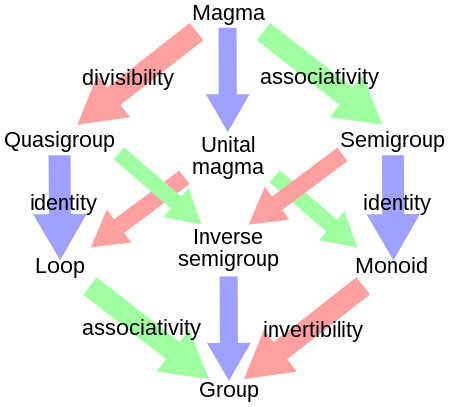
\includegraphics[width=0.7\textwidth]{figures/Sample/Magma_to_group.jpg}
	\caption{Algebraic structure hierarchy \cite{enwiki:1107380309}}
	\label{fig_magma}
 \end{figure}
The definitions of constructs like homomorphism and direct product is given to
us by universal algebra. Universal algebra provides a common framework by
abstracting out the specific definitions and properties of algebraic structures.
It helps us to study the commonalities of algebraic structures and define their
constructs. An algebra in universal algebra is defined as an ordered pair
$(S,F)$ where $S$ is a set and $F = (F_i:i\in I)$ is a finitary operations on A
for some indexing set $I$ \cite{sannella2012foundations}. Certain constructs
like morphisms and direct products help us to relate different mathematical
objects and structures in a systematic and rigorous way. Morphisms
allow us to understand how different algebraic structures are related to one
another. Direct product, on the other hand, is a useful tool for combining
structures, such as monoids, groups, or rings, to create new and more
complex structures that retain many of the desirable properties of the original
structures. This allows us to study and understand larger, more complex systems
and their properties.

\section{Research Outline}
To define the scope of our research to study algebraic structures in proof
assistant systems, we capture the current coverage of algebraic structures in
the standard libraries of these systems. As part of the survey, we consider four
libraries: The Agda standard library (v1.7.1), the mathematical component
library (1.12.0) for Coq, Idris 2, and mathematical library for Lean 3. In
the effort of finding the coverage of algebraic structures in these libraries, we
develop a clickable table that directs to the definition of the structure in the
source code of these systems. Through the survey, we establish our focus for
contributing to the Agda standard library\footnote{I was exposed to Agda during
coursework for my Master's degree, further adding bias to choosing Agda over
other systems}.

Inspired by the ways algebraic structures are used in research, in this work we
explore capturing a select subset of them in the Agda standard library.
Following the algebra hierarchy in Figure ~\ref{fig_magma}, we study magma with
division operation that is quasigroup and loop structures. By defining them with
their morphisms and direct product constructs, we can study their properties and
relationships in a more systematic way. We also explore various types of loops
such as bol-loop and moufang-loop and their properties. Semigroups are used in
various fields such as probability theory and formal systems. One of the most
commonly studied algebraic structure is Ring. In this thesis, we study types of
rings such as near-ring, quasi-ring, and non-associative ring. Another commonly
used structure that has its applications in various fields is Kleene algebra.
The applications of Kleene algebra are seen in finite state machines, regular
expressions, and other branches of computer science. As part of this thesis, we
study Kleene algebra by providing proof for its properties that may be used in
developing other systems or applications. By contributing to Agda standard
library, we hope that this work will be used by others. 

As we explore capturing these structures in Agda, we encountered several
problems. In this work, we abstract out these problems into five classes:
\begin{enumerate}
\item Ambiguity in naming structures.
\item Equivalent structures that are structurally different.
\item Redundant field during structural inheritance.
\item Identical structures that can be derived in many ways in algebra hierarchy
\item Equivalent structures that are structurally the same.
\end{enumerate}
We analyze each problem and provide plausible solutions whereever possible.

\section{Thesis Outline}
Chapters 2 and 3 focus on the background information necessary for reading this
work, focusing on reviewing universal algebra and algebraic structures in Agda,
respectively. Chapter 4 justifies the scope of the thesis contribution through a
survey on algebraic coverage in proof systems. The next three chapters 5,6 and 7
are dedicated to discussing the structures in detail. Chapter 5 explores
quasigroup and loop structures that use division operation. Chapter 6 discusses
the properties of semigroup and ring with variations of the ring structure. Chapter
7 explores Kleene algebra, definition, construct and properties in Agda. Chapter
8 describes the various problems we faced during this work, as well as advice on
handling common issues in programming algebras in proof systems. Finally,
Chapter 9 concludes this work with notes on related future works and some
closing thoughts.
